\documentclass[]{article}

\usepackage{tikz}
\usepackage{amsmath}
\usepackage{amsfonts}
\usepackage{amssymb}
\usepackage{relsize}
\usepackage{tkz-base}
\usepackage{tkz-euclide}

\usetikzlibrary{svg.path}
\usetikzlibrary{arrows}
\usetikzlibrary{shapes.geometric,calc}

\newcommand{\crossout}[1]{\mathbin{\ooalign{${#1}$\cr\larger[1]{$\nearrow$}\cr}}}

%opening
\title{Inverse Kinematics II}
\author{Glen Henshaw\\Craig Carignan}



\begin{document}

\maketitle


\section{Numerical Inverse Kinematics}
It's often difficult to impossible to find a closed--form solution for the inverse kinematics of a given manipulator. But it's always possible to solve the inverse kinematics problem numerically. This has become more popular in the last decade or so because embedded computers have become powerful enough to enable it.

Numerical techniques are also often more flexible and powerful than closed--form techniques. A good numerical approach can be agnostic to the manipulator kinematics, for instance; you can give it the DH parameters of whatever arm you are using, and it will work with few changes. You can even add or subtract degrees of freedom.

\section{Direct Numerical Search}
You might be tempted to just set this up as a problem in joint space:
\begin{displaymath}
\min_{\underline{q}}\ \|\ \!^{O}_{W}T - ^{0}T(\underline{q})\|
\end{displaymath}
or similar. This minimization problem could in theory be solved by gradient descent or a quasi--Newton method.

This \textbf{can} work, but it often doesn't. The issue is that the minimization problem is nonlinear, and hence may have many locally minima. In general it has no special structure that lends itself to being solved by nonlinear optimization solvers. It is also difficult to bound the number of iterations needed to find the solution, and hence in realtime applications it can be problematic.

\section{Jacobian--based Techniques: Resolved--motion Rate Control (RMRC)}
A better idea is to think about the problem in terms of Cartesian velocities and rates instead of positions and orientations. That lets us use the fact that the Jacobian relationship:
\begin{displaymath}
\dot{\underline{x}} = J(\underline{q})\dot{\underline{q}}
\end{displaymath}
is linear with respect to the joint rates $\dot{\underline{q}}$. The problem, of course, is that the Jacobian relationship goes the wrong way. We want to be able to fix $\dot{\underline{x}}$ and calculate $\dot{\underline{q}}$.

You could consider just inverting the Jacobian:
\begin{displaymath}
\dot{\underline{q}} = J^{-1}(\underline{q})\dot{\underline{x}}
\end{displaymath}
This is also, generally speaking, a bad idea. The most obvious problem is that the Jacobian may not even be square: it is $N \times 6$, where $N$ is the number of degrees of freedom of the manipulator. So if your manipulator is not 6--DOF, you \textit{can't} take an inverse. But even if you do have a 6--DOF manipulator, simply inverting the Jacobian is a bad idea, because square matrices can be singular. So we'll talk about what it means, both mathematically and mechanically, to have a singular Jacobian.
 
 \subsubsection{An aside: some concepts from linear algebra}
Consider the system
\begin{displaymath}
Ax=0
\end{displaymath}
where $A$ is any matrix, square or nonsquare. If $A$ is $M$ by $N$, the set of all vectors $X$ that satisfy this equation form a subset of $\mathbb{R}^{N}$. This subset is nonempty, since it clearly contains the zero vector: $x = 0$ always satisfies $A x = 0$. This subset actually forms a subspace of $\mathbb{R}^{N}$, called the \textit{nullspace} of the matrix $A$ and denoted $N(A)$. If $x_{1}$ is in $N(A)$, then, by definition, $A(x_{1}+x_{2}) = Ax_{2}$ for any value of $x_{2}$. 

In terms of robotic manipulators, the Jacobian will always have a nullspace. For a 6--DOF manipulator, in general the nullspace will contain only the zero vector. But for a manipulator with more than 6 DOF, the nullspace will contain a subspace of joint rates \textbf{that do not cause the end effector to move}. In other words, for nearly any arm pose $\underline{q}$, you will be able to find an infinite number of joint rate vectors $\dot{\underline{q}}$ such that $J(\underline{q})\dot{\underline{q}} = 0$.

This is called ``self--motion''. It is perhaps easiest to visualize with a 7--DOF revolute arm: in this case, you can independently choose to rotate the elbow without moving the end effector.

If $A$ is square, it may or may not be invertible. A square matrix $A$ that is not invertible is called \textit{singular}. This means that there exists at least some vector $\underline{x} \in \mathbb{R}^{N}$ not equal to zero such that $A\underline{x}=0$. A matrix that is singular may also be referred to as a reduced--rank matrix, as distinguished from a full-rank matrix. Although the formal mathematical concept of singularity is only defined for square matrices, in robotics we use this term somewhat loosely. We will say that a nonsquare $M \times N$ matrix that has a row rank less than $N$ is also singular.

Physically, when we refer to a singular Jacobian, what this means is that the arm is in a pose where it cannot produce a Cartesian tooltip velocity in some direction. Recall that the standard (read: bad) way of calculating an inverse that is taught in linear algebra courses involves dividing by the matrix determinant. A singular matrix has a determinant of 0, so attempting to calculate the inverse of a singular matrix is the linear algebra equivalent of a divide--by--zero.

Consequently, if you blindly stuff a singular Jacobian into any sort of numerical inversion routine, in the best case you will end up with infinite values for at least some of the matrix entries (assuming your code doesn't just blow up!), and if you then multiply it by a desired Cartesian tooltip velocity vector, you may end up with infinitely large joint rates.

\section{Manipulability and Singularities}
The \textit{manipulability} of a manipulator is (usually) a function of its pose, and refers to how close the Jacobian is to becoming reduced--rank. A manipulator is in a singular pose when the Jacobian at that pose does, in fact, become reduced--rank. There are several ways of calculating the manipulability of a robotic arm. One way is to examine the determinant of the Jacobian; there are at least three or four other widely used techniques.

Singular poses have the following characteristics:
\begin{itemize}
	\item mobility of the manipulator is reduced
	\item infinite numbers of solutions to the inverse kinematics may exist
	\item small desired end effector velocities may result in very large joint velocities
	\item small joint torques may cause very large tool tip forces
\end{itemize}

There are two types of singularities: \textit{boundary singularities} and \textit{internal singularities}. Boundary singularities are poses where the tooltip lies on the boundary of the workspace. Remember our diagram from last lecture:
\begin{figure}[h!]
	\centering
	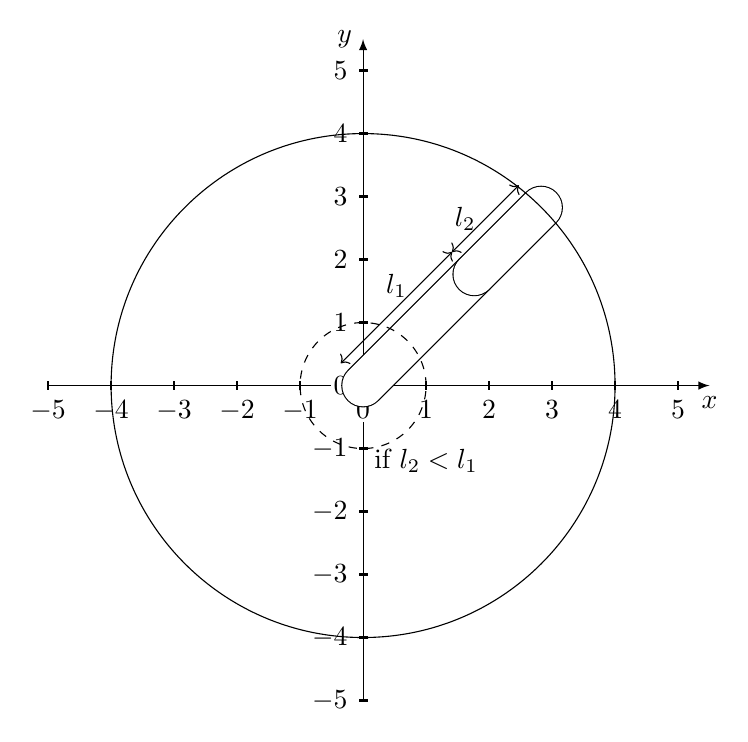
\begin{tikzpicture}[scale=0.8]
	\tkzInit[xmax=5,ymax=5,xmin=-5,ymin=-5]
	\tkzAxeXY
	
	\draw[cm={0.707,0.707,-0.707,0.707,(0,0)}][double=none, double distance=15pt, line join=round, line cap=round] (0.0, 0.0) -- (2.5, 0);
	\draw[cm={0.707,0.707,-0.707,0.707,(0,0)}][<->] (0, 0.5) -- (2.5, 0.5) node[above][pos=0.5]{$l_{1}$};	
	
	\draw[cm={0.707,0.707,-0.707,0.707,(1.765, 1.765)}][double=none, double distance=15pt, line join=round, line cap=round] (0.0, 0.0) -- (1.5, 0);
	\draw[cm={0.707,0.707,-0.707,0.707,(1.765, 1.765)}][<->] (0, 0.5) -- (1.5, 0.5) node[left][pos=0.5]{$l_{2}$};
	\draw (0,0) circle (4.0cm);
	\draw[dashed] (0,0) circle (1.0cm) node at (1,-1.2) {$\text{if } l_{2}<l_{1}$};
	\end{tikzpicture}
\end{figure}
except here the arm is full stretched out so that the end effector lies exactly on the outer workspace boundary. This arm is in a singular pose, and cannot produce a Cartesian velocity along the direction orthogonal to the normal of the workspace (either inward or outward). All robotic arms have singular poses at their workspace boundaries.

For many manipulators there are also poses that are not on a workspace boundary where the manipulator cannot produce a velocity in some direction. It's important to avoid these situations. Some ways to locate such poses:
\begin{itemize}
	\item Set the determinant to zero, $|J(\underline{q})|=0$, and solve for $\underline{q}$
	\begin{itemize}
		\item only works for 6--DOF  arms (or other arms with square Jacobians)
		\item this is essentially an exhaustive search; there may be many such poses, and you have to somehow find all of them.
	\end{itemize}
	\item Examine the rank degeneracy of $J$. If we express the Jacobian as
	\begin{displaymath}
	J = \left[\begin{array}{ccccc} | & | & | & | & | \\ c_{1} & c_{2} & c_{3} & \cdots & c_{N} \\ | & | & | & | & |\end{array}\right]
	\end{displaymath}
	then $J$ becomes deficient when the $c$ vectors become linearly dependent.
	
	Note that for an arm with a spherical wrist, this can be split into two subproblems: $J_{tran}(\theta_{arm})$ and $J_{rot}(\theta_{wrist})$.
\end{itemize}

\subsection{Example: two axis planar arm}
\begin{figure}[h!]
	\centering
	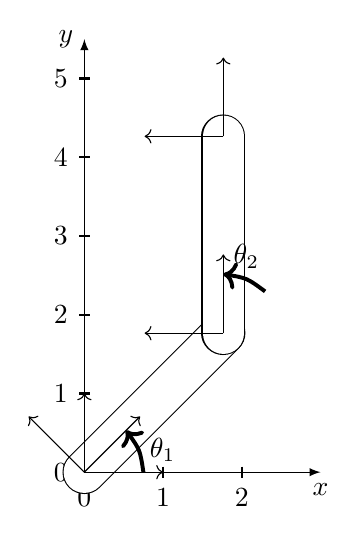
\begin{tikzpicture}
	\tkzInit[xmax=2.5,ymax=5,xmin=0,ymin=0]
	%\tkzGrid
	\tkzAxeXY
	\draw[cm={0.707,0.707,-0.707,0.707,(0,0)}][double=none, double distance=15pt, line join=round, line cap=round] (0.0, 0.0) -- (2.5, 0);
	\draw[cm={0.707,0.707,-0.707,0.707,(0, 0)}][->] (0.0, 0.0) -- (1.0, 0.0);
	\draw[cm={0.707,0.707,-0.707,0.707,(0, 0)}][->] (0.0, 0.0) -- (0.0, 1.0);
	\draw[cm={0.707,0.707,-0.707,0.707,(0, 0)}][line width=0.5mm][<-] (.75, 0.0) .. controls (0.7, -0.3) .. (0.75*0.707, 0.75*-0.707)  node[pos=0.5,right]{$\theta_{1}$};
	
	\draw[cm={0, 1, -1, 0,(1.765, 1.765)}][double=none, double distance=15pt, line join=round, line cap=round] (0.0, 0.0) -- (2.5, 0);
	\draw[cm={0, 1, -1, 0,(1.765, 1.765)}][->] (0.0, 0.0) -- (1.0, 0.0);
	\draw[cm={0, 1, -1, 0,(1.765, 1.765)}][->] (0.0, 0.0) -- (0.0, 1.0);
	\draw[cm={0, 1, -1, 0,(1.765, 1.765)}][line width=0.5mm][<-] (.75, 0.0) .. controls (0.7, -0.3) .. (0.75*0.707, 0.75*-0.707) node[pos=0.5,above]{$\theta_{2}$};
	
	\draw[->] (0.0, 0.0) -- (1.0, 0.0);
	\draw[->] (0.0, 0.0) -- (0.0, 1.0);
	
	\draw[cm={0, 1, -1, 0, (1.765, 4.265)}][->] (0.0, 0.0) -- (1.0, 0.0);
	\draw[cm={0, 1, -1, 0, (1.765, 4.265)}][->] (0.0, 0.0) -- (0.0, 1.0);

	\end{tikzpicture}
	\caption{Two--link planar manipulator}
\end{figure}

We're going to use the simplest $J$, which we derived a couple of lectures ago, in order to make life easier on ourselves. Jacobians expressed in different frames all have exactly the same singularities, so we are free to use the Jacobian expressed in any frame we like.
\begin{displaymath}
^{3}J = \left[ \begin{array}{cc} l_{1}s_{2} & 0 \\ l_{1}c_{2}+l_{2} & l_{2} \end{array}\right]
\end{displaymath}
where $M=2\ \ (x,y)$ and $N=2\ \ (\theta_{1}, \theta_{2})$.

Setting the determinant to zero:
\begin{displaymath}
|J| = l_{1}l_{2}s_{2} = 0 \Rightarrow \theta_{2} = 0^{\circ}\ \text{or}\ 180^{\circ}
\end{displaymath}
in which case,
\begin{displaymath}
^{3}J = \left[ \begin{array}{cc} 0 & 0 \\ l_{1}+l_{2} & l_{2} \end{array}\right]
\end{displaymath}
and the two columns are not linearly dependent.

\subsubsection{Joint velocities near the singularity}
\begin{displaymath}
	\dot{\underline{q}} = \ \!^{3}J^{-1}\ \!^{3}\underline{x} \Rightarrow \ \!^{3}J^{-1} = \left[\begin{array}{cc} \frac{1}{l_{1}s_{2}} & 0 \\ -(\frac{1}{l_{1}s_{2}} + \frac{c_{2}}{l_{2}c_{2}}) & \frac{1}{l_{2}} \end{array}\right]
\end{displaymath}
so
\begin{eqnarray}
	\dot{\theta_{1}} & = & \frac{1}{l_{1}s_{2}}\dot{x} \nonumber\\
	\dot{\theta_{2}} & = & -\left(\frac{1}{l_{1}s_{2}} + \frac{c_{2}}{l_{2}s_{2}}\right)\dot{x} \nonumber
\end{eqnarray}
which implies that the arm cannot move in the $y$ direction, and an attempt to set $\dot{\underline{x}}$ will result in the denominators of the fractions becoming zero, hence the joint rates will become infinite.

\textbf{NOTE, however} that even if $\theta_{2}$ is not exactly $0^{\circ}$ or $180^{\circ}$ but is merely close to one of these values, the denominators of the expressions will be quite large. Hence, the singularity is ``felt'' for some distance away; exactly how far depends on the maximum joint rates that are acceptable and/or achievable.

\subsubsection{End Effector forces near the singularity}
\begin{displaymath}
^{3}\underline{f} = \ \!^{3}J^{-T}\underline{\tau}
\end{displaymath}
so
\begin{eqnarray}
	f_{x} & = & \frac{1}{l_{1}s_{2}}\tau_{1} - \left(\frac{1}{l_{1}s_{2}} + \frac{c_{2}}{l_{2}s_{2}}\right) \tau_{2} \nonumber \\
	f_{y} & = & \frac{1}{l_{2}}\tau_{2} \nonumber
\end{eqnarray}
which implies that $f_{x} \rightarrow \infty$ near the singularity.

\subsection{Example: PUMA RRR Wrist}
The D--H table for the PUMA robot wrist is
\begin{figure}[h!]
	\centering
	\begin{tabular}{c|cccc}
		i & $\alpha_{i-1}$ & $a_{i-1}$ & $d_{i}$ & $\theta_{i}$ \\ \hline
		4 & $-90^{\circ}$ & $\alpha_{3}$ & $d_{4}$ & $\theta_{4}$ \\
		5 & $+90^{\circ}$ & $0$ & $0$ & $\theta_{5}$ \\
		6 & $-90^{\circ}$ & $0$ & $0$ & $\theta_{6}$
	\end{tabular}
\end{figure}
\begin{displaymath}
	^{3}J_{rot} = \left[\begin{array}{ccc} 0 & s_{4} & -c_{4}s_{5} \\ 1 & 0 & c_{5} \\ 0 & c_{4} & s_{4}s_{5} \end{array}\right]
\end{displaymath}
\begin{displaymath}
|\ \!^{3}J| = -\sin{\theta_{5}} \Rightarrow \theta_{5} = 0^{\circ}, \pm 180^{\circ}
\end{displaymath}
At the singularity,
\begin{displaymath}
^{3}J_{rot} = \left[\begin{array}{ccc} 0 & s_{4} & 0 \\ 1 & 0 & 1 \\ 0 & c_{4} & 0 \end{array}\right]
\end{displaymath}
so the first and third columns are linearly dependent. At the singularity, the first roll axis is aligned with the third roll axis, and essentially they have become redundant.

This is an important point: interior singularities occur at poses where degrees of freedom that are normally independent become redundant.

\subsection{Pseudo--inverses} 
OK, so if taking a direct inverse of the Jacobian is a bad idea, what else can we do? A better idea is to use a pseudo--inverse. Contrary to popular opinion, there are in general an infinite number of pseudo--inverses for a matrix, but the one everyone knows about is the Moore--Penrose pseudo--inverse:
\begin{displaymath}
	J^{\dag} \triangleq J^{T}\underbrace{(JJ^{T})}_{square!}\ \!\!^{-1}
\end{displaymath}
You can always take a Moore--Penrose pseudo--inverse, even for a nonsquare Jacobian. In addition, the Moore--Penrose pseudo--inverse has the nice property that it minimizes the 2--norm:
\begin{displaymath}
	\| J^{\dag}(\underline{q})\dot{\underline{x}} \|_{2}^{2} = \min \| \dot{\underline{q}} \|_{2}^{2}\ \text{ s.t. } J(\underline{q})\dot{\underline{q}} = \dot{\underline{x}}
\end{displaymath}
What this means is that of all the vectors of joint rates that lie in the nullspace of the Jacobian, the Moore--Penrose pseudo--inverse finds the one that is smallest, e.g. the joints rates are the lowest.

To tie this into our aside above: any given pseudo--inverse will choose exactly one joint rate vector $\dot{\underline{q}}_{2}$ that satisfies $\dot{\underline{x}} = J(\underline{q})\dot{\underline{q}}_{2}$. But if the Jacobian has a nontrivial nullspace $N(J)$, we can find an infinite number of vectors $\dot{\underline{q}}_{1}$ such that $\dot{\underline{x}} = J(\underline{q})(\dot{\underline{q}}_{2} + \dot{\underline{q}}_{1})$. The Moore--Penrose pseudo--inverse inherently chooses $\dot{\underline{q}}_{1}$ such that  $\| \dot{\underline{q}}_{1} + \dot{\underline{q}}_{2} \|_{2}^{2}$ is the smallest it can be.

There are more clever ways to pick $\dot{\underline{q}}_{1}$. You could, for instance, choose a $\dot{\underline{q}}_{1}$ that moves the elbow of your arm away from a potential collision hazard or that improved its manipulability.

One easy way to improve the robustness of any technique that uses a Moore--Penrose pseudo--inverse is to add what is called a \textit{damped least--squares} term:
\begin{displaymath}
J^{\dag} \triangleq J^{T}(JJ^{T} + \gamma I)\ \!\!^{-1}
\end{displaymath}
where $\gamma \ll 0$. Equivalently, this adds a small positive value to the diagonal of the square matrix that is being inverted. The effect of this is to limit joint rates in the vicinity of a singularity, so it adds singularity robustness. The tradeoff for this is that the trajectory the arm takes will deviate somewhat from the (impossible to follow) trajectory that you specified.

A different, more mathematically justifiable, way to robustly take a pseudo--inverse is based on the singular--value decomposition (SVD). SVDs are beyond the scope of this course, but if you already know about SVDs, the idea is that the ``singular values'' of a matrix, which are sort of like eigenvalues, can be used to directly compute the matrix inverse. A near--singular matrix will have a number of singular values that are very small. You can simply drop these singular values and only use the ones that are above some threshold to calculate a pseudo--inverse.

\subsection{Problems with pseudo--inverses}
First, it's important to bear in mind that a manipulator singularity is a mechanical phenomenon. Better math won't let us get rid of singularities. So even if you use a Moore--Penrose pseudo--inverse, if the arm is in a singular pose, you still won't be able to move it along its singular direction. Your best bet is to avoid singular poses somehow, normally by examining the rank of the Jacobian --- or some other manipulability index --- along the trajectory you want and if it starts to become singular, modify the trajectory.

A more subtle problem stems from the fact that we're operating in joint velocity space. In order to get back to joint angle space, i.e. to have something useful to send to whatever control laws are controlling the actuators: we have to perform an integration.

Numerical integrators are susceptible to drift. Simple ones that are suitable for realtime use are especially so. If you do something like
\begin{displaymath}
\underline{q}_{i+1} = \underline{q}_{i} + J^{\dag}(\underline{q}_{i})\dot{\underline{x}}
\end{displaymath}
i.e. use a straight forward Euler integration scheme, you will get trajectories that look like this:

\begin{figure}[h!]
	\centering
	\begin{tikzpicture}
	\draw (0,0) .. controls (1,-0.5) and (2,3.5) .. (3,3) node[right] {desired};
	\draw[rotate=-15,dotted] (0,0) .. controls (1,-0.5) and (1.8,3.2) .. (2.2,2.8) node[right] {actual};
	\end{tikzpicture}
\end{figure}
There are two common ways to solve this. 

\subsubsection{Iterated Jacobian method}
One is called the ``iterated Jacobian method''. The idea is that you do a Newton--Raphson iteration on \textit{position}.
\begin{eqnarray}
	\underline{x} & = & \underline{f}(\underline{q}) \nonumber \\
	\underline{x}_{0} & = & \underline{f}(\underline{q_{0}}) \nonumber
\end{eqnarray}
Take a Taylor series about $\underline{q}_{0}$:
\begin{eqnarray}
	\underline{f}(\underline{q}_{0}+\Delta \underline{q}) & = & \underline{f}(\underline{q}_{0}) + \left.\frac{\partial \underline{f}}{\partial\underline{q}}\right\rvert_{\underline{q}=\underline{q}_{0}}\!\!\!\!\Delta \theta + O(\Delta \underline{q}^{2}) \nonumber \\
	%\underline{x} & = & \underline{x}_{0} + J(\underline{q}_{0})(\underline{q}-\underline{q}_{0}) \Rightarrow \nonumber \\
	\underline{q} & = & \underline{q}_{0}+J^{\dag}(\underline{q}_{0})\underbrace{\left[\underline{x}-\underline{x}_{0}\right]}_{\Delta\underline{x}}\ \ \ \ \ \text{for}\ N=M
\end{eqnarray}
Note that $\Delta x$ must be small for this to converge.

OK, what is $\underline{x}$ here? 
\begin{displaymath}
\underline{x} = \left[ \begin{array}{c} \underline{p} \\ \\? \end{array}\right]
\end{displaymath}
$\underline{p}$ is straightforward: It's your Cartesian position vector. But what is in the rotation spot?

It depends on how you have chosen to represent orientation, \textbf{but it must be a three--parameter representation}. If you are using Euler or fixed angles, it can be simply those. But if it's a quaternion, you have a bit of a problem, because quaternions have four parameters. Remember, though, that quaternions are defined as 
\begin{displaymath}
	\underset{\sim}{q} = \left[ \begin{array}{c} \psi \\ \hat{n} \end{array} \right]
\end{displaymath}
where $\psi$ is a scalar and $\hat{n}$ is a 3--vector. \textbf{In a small angle situation}, $\psi$ is close to unity and $\hat{n}$ is close to zero, and exactly zero if the angle is zero. In fact, for small angles, $\hat{n}$ approximates $1/2$ time the 3--2--1 Euler angles.  In general we use $\hat{n}$ as the rotation part.

So what's $\Delta \underline{x}$? Again, for the positional part it's straightforward: it's $\underline{p}-\underline{p}_{0}$. And again, for rotation... it's complicated.

If you are using an Euler angle or fixed angle set, you can subtract them. This hand--waves over a bunch of math but as a small angle approximation it holds, and only extreme pedants (or possibly those cramming fo their doctoral quals) need go any further. So if you are using the $\left[\alpha, \beta, \gamma\right]^{T}$ set:
\begin{displaymath}
\underline{x} = \left[ \begin{array}{c} \underline{p} \\ \alpha-\alpha_{0} \\ \beta-\beta_{0} \\ \gamma-\gamma_{0} \end{array}\right]
\end{displaymath}

If you are using a quaternion representation, you really shouldn't just subtract $\hat{n}$ from $\hat{n}_{0}$. The proper way to calculate the difference between two quaternions $\underset{\sim}{q}$ and $\underset{\sim}{q}_{0}$ is:
\begin{displaymath}
\underset{\sim}{q}\ \!\!_{0} * \Delta {\underset{\sim}{q}} = \underset{\sim}{q}\ \Rightarrow\ \Delta {\underset{\sim}{q}} = \underset{\sim}{q} * \underset{\sim}{q}\ \!\!_{0}^{-1}
\end{displaymath}
and it turns out that the quaternion inverse is
\begin{displaymath}
{\underset{\sim}{q}}^{-1} = \left[\begin{array}{c} \psi \\ - \hat{n} \end{array}\right]
\end{displaymath}
and quaternion multiplication is defined as
\begin{displaymath}
	\left[\begin{array}{c} \psi_{1} \\ - \hat{n}_{1} \end{array}\right] \times \left[\begin{array}{c} \psi_{2} \\ - \hat{n}_{2} \end{array}\right] = \left[\begin{array}{c} \psi_{1}\psi_{2} - \hat{n}_{1}\cdot\hat{n}_{2} \\ \psi_{1}\hat{n}_{2} + \psi_{2}\hat{n}_{1} + \hat{n}_{1} \times \hat{n}_{2} \end{array}\right]
\end{displaymath}


So the algorithm is then:
\begin{itemize}
	\item[1] $\underline{q}_{0}=\underline{q}$ and $\underline{x}_{0} = \underline{f}(\underline{q})$
	\item[2] $\Delta\underline{x} = \underline{x}$``-''$\underline{x}_{0}$
	\item[3] $J=J(\underline{q})$
	\item[4] $\Delta \underline{q} = J^{\dag}\Delta \underline{x}$
	\item[5] $\underline{q} = \underline{q}_{0} + \Delta \underline{q}$
	\item[6] $\|\Delta \underline{q}\| < \epsilon$? If yes, stop
	\item[7] go to 1
\end{itemize}

\subsubsection{Direct Error Correction}
Another way to solve the integral drift problem is simply to build an error correction term into the RMRC law, e.g. to implement
\begin{displaymath}
\dot{\underline{q}} = J^{\dag}(\underline{q})\left(\dot{\underline{x}} + \gamma \Delta \underline{x}\right)
\end{displaymath}
where $\gamma$ is a gain that has to be selected for good performance, and everything else is defined as we did above.
\subsubsection{Constrained quadratic optimization}
It turns out that we can derive a straightforward quadratic optimization problem in the spirit of RMRC:
\begin{eqnarray}
&&\min_{\dot{\underline{q}}} \ \ \|\dot{\underline{x}} - J(\underline{q})\dot{\underline{q}}\|^{2} \nonumber \\
& = & \min_{\dot{\underline{q}}}\ \ \left( \dot{\underline{x}} - J(\underline{q})\dot{\underline{q}} \right)^{T}\left( \dot{\underline{x}} - J(\underline{q})\dot{\underline{q}} \right) \nonumber \\
& = & \min_{\dot{\underline{q}}}\ \ \dot{\underline{x}}^{T}\dot{\underline{x}} - 2\dot{\underline{x}}^{T}J(\underline{q})\dot{\underline{q}} + \dot{\underline{q}}^{T}J^{T}(\underline{q})J(\underline{q})\dot{\underline{q}} \nonumber \\
& = & \min_{\dot{\underline{q}}}\ \ -2\dot{\underline{x}}^{T}J(\underline{q})\dot{\underline{q}} + \dot{\underline{q}}^{T}J^{T}(\underline{q})J(\underline{q})\dot{\underline{q}} \nonumber
\end{eqnarray}
This is in a form for which there are many good, realtime--capable quadratic optimization solvers. unlike the two previous techniques, though, in this form it's easy to add constraints, e.g.
\begin{eqnarray}
&& \min_{\dot{\underline{q}}}\ \ -2\dot{\underline{q}}^{T}J(\underline{q}) + \dot{\underline{q}}^{T}J^{T}(\underline{q})J(\underline{q})\dot{\underline{q}} \nonumber \\
&&\text{s.t.} \nonumber \\
&&-\theta_{1,min} \le \theta_{1} \le \theta_{1,max} \nonumber \\
&&-\theta_{2,min} \le \theta_{2} \le \theta_{2,max} \nonumber \\
&&\vdots \nonumber
\end{eqnarray}
and with a little cleverness you can even add constraints that depend on $\underline{q}$, not $\dot{\underline{q}}$, such as collision constraints. You can also correct for integrator drift by solving
\begin{eqnarray}
&& \min_{\dot{\underline{q}}} \ \ \|\dot{\underline{x}} - J(\underline{q})\dot{\underline{q}}\|^{2} + \gamma \| \underline{q}_{d} - \left(\underline{q} + \Delta t \dot{\underline{q}} \right) \| ^{2} \nonumber 
\end{eqnarray}

Thinking along these lines eventually leads you to a technique called model--predictive control, which if you've ever seen YouTube videos of robots doing parkour, you've seen in action. It is a very powerful technique for robotic motion control.
\end{document}
